\subsection{Semi-automatic modeling for gene regulatory networks}
Within his masters dissertation, Matthew
Kondoff~\cite{kondoff2015modeling} looked at a way of automatically
generating computational models from human-readable description of
regulatory gene networks. His efforts resulted in an R package, with
the help of which a convenient way of numerical modeling was
providing, thus hiding the low-level nitty-gritty of translating the
network description into formulas and computer code.

\begin{figure}
\begin{center}
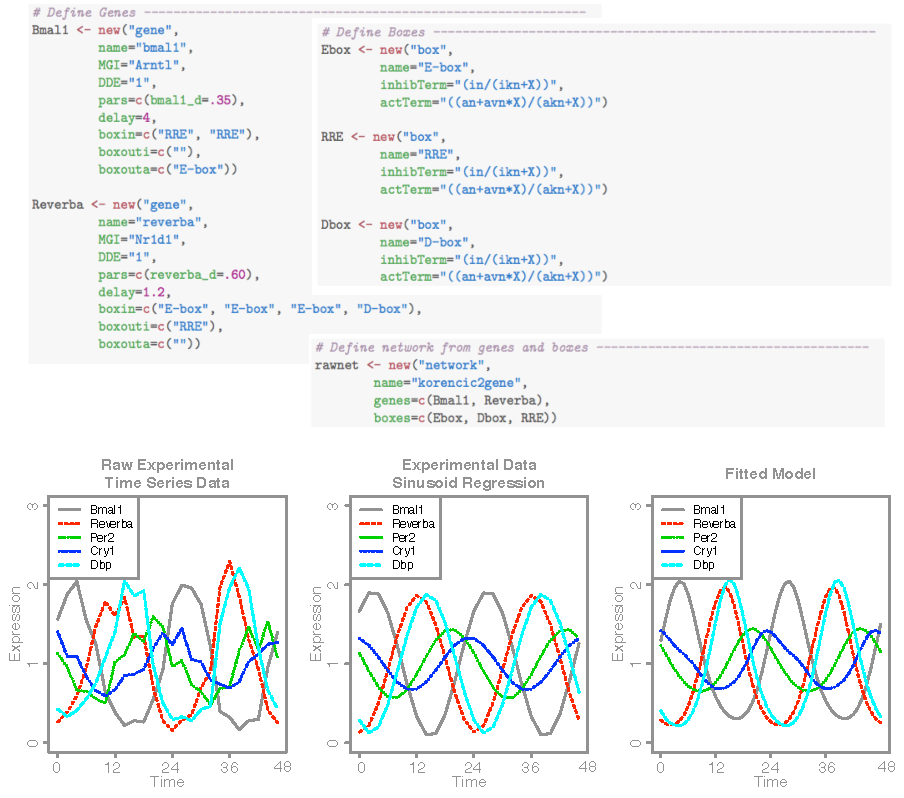
\includegraphics[width=\linewidth]{figures/matt/matt.pdf}
\end{center}
\caption{
  {\bf Upper panel} An example of a human-readable description of a
  gene regulatory network consisting of two genes (Bmal1 and
  Reverb$\alpha$) and three boxes (Ebox, RRE, Dbox).
  {\bf Lower panel} Comparison between oscillations in microarray
  data, the extracted first harmonic and the fit by a model with five
  genes.
\label{fig::matt}
}
\end{figure}


Used~\cite{zhang2014circadian} microarray data to verify and fit the
parameters of the numerical model.

